\باب{تغیری اصول}\شناخت{باب_تغیری_اصول}

\حصہ{نظریہ}
فرض کریں آپ ایک نظام جس کو ہیملٹنی H بیان کرتا ہو٬ کی زمینی حال توانائی
 \(E_{gs}\)
  کا حساب کرنا چاہتے ہیں لیکن آپ غير تابع وقت شروڈنگر مساوات حاصل کرنے سے قاصر ہوتے ہیں . اصول تغيوریت آپ کو 
 \(E_{gs}\)
  کی بالائی حد دیتا ہے . بعض اوقعات آپ کو صرف اسی سے غرض ہوتا ہے اور عموماً ہوشیاری سے کام لیتے ہوئے آپ بالکل ٹھیک قیمت کے قريب قیمت حاصل کر سکتے ہیں . آئیں اس کا استعمال دیکھے. کوئی بھی معمول شده تفاعل 
\(\psi\)
  لیں ۔ میں درج ذيل دعوه کرتا ہوں:
\[E_{gs}\le \langle \psi |H|\psi\rangle \equiv \langle H \rangle\]
یعنی کسی بھی شائد غير درست حال 
\(\psi\)
 میں H کی توقعاتی قیمت زمینی حال توانائی سے زياده ہوگی. یقیناً اگر 
 \(\psi\) 
 اتفاقاً ایک ہیجان حال ہو تب H کی قیمت
 \(E_{gs}\) 
 سے تجاوز کرے گی. اصل نقطہ یہ ہے کہ کسی بھی تفاعل 
 \(\psi\)
 کے لیے بھی ایسا ہوگا.\\
ثبوت: \\
چونکہ H کے نامعلوم امیتازی تفاعلات مكمل سلسلہ دیتے ہیں. لحاظہ ہم 
\(\psi\) 
کو ان کا خطی جوڑ لکھ سکتے ہیں.\\
جہان
\[\psi=\sum c_{n}\psi_{n}, \quad H\psi_{n}=E_{n}\psi_{n}\] 
ہے .چونکہ 
\(\psi\) 
معمول شده ہے\\
\[1=\langle \psi |\psi\rangle=\big\langle \sum_{m} c_{m}\psi_{m}|\sum_{n}c_{n}\psi_{n}\big\rangle=\sum_{m}\sum_{n}c_{m}^{*}c_{n}\langle \psi_{m}|\psi_{n}\rangle=\sum_{n}\abs{c_{n}}^{2}\]
جہاں فرض کیا گیا ہے کے امتیازی تفاعلات از خد معیاری معمول شدہ ہے.
\[\langle \psi_{m}|\psi_{n}\rangle=\delta_{mn}\]
ساتھ ہی درج ذیل ہوگا
\[\langle H \rangle=\big\langle \sum_{m} c_{m}\psi_{m}|H\sum_{n}c_{n}\psi_{n}\big\rangle=\sum_{m}\sum_{n}c_{m}^{*}E_{n}c_{n}\langle \psi_{m}|\psi_{n}\rangle=\sum_{n}E_{n}\abs{c_{n}}^{2}\]
ليكن تعريف کی رو سے زمینی حال توانائی کم سے کم امتیازی قیمت ہوگی. لحاظہ
\(E_{gs}\le E_{n}\)
ہوگا. جس کے تحط درج ذیل ہوگا
\[\langle H \rangle \ge E_{gs}\sum_{n}\abs{c_{n}}^{2}=E_{gs}\]
جس کو ہم ثابت کرنا چاہتے تھے.\\
مثال \\7.1
فرض كرے ہم یک بودی ہارمونی مورتیش
\[H=-\frac{\hbar^{2}}{2m}\frac{\dif^{2}}{\dif{x^{2}}}+\frac{1}{2}m\omega^{2}x^{2}\]
کی زمینی حال توانائی جاننا چاہتے ہیں . یقیناً ہم اس کا ٹھیک ٹھیک جواب جانتے ہیں. جو مساوات 2.61
\(E_{gs}=(1/2)\hbar\omega\)
جسے استعمال کرکے اس ترقيب کو پرکا جاسکتا ہے. ہم گاوسی تفاعل
 \[\psi(x)=Ae^{-bx^{2}}\] 
کو اپنا پرکیا تفاعل موج منتخب کرتے ہے جہاں b ایک مستقل ہے اور A کو معمول زنی سے تعائن کیا جاسکتا ہے.
\[1=\abs{A}^{2}\int_{-\infty}^{+\infty}e^{-2bx^{2}}\dif{x}=\abs{A}^{2}\sqrt{\frac{\pi}{2b}}\Rightarrow \big (\frac{2b}{pi}\big )^{1/4}\]
اب درج ذیل ہے
 \[ \langle H \rangle=\langle T \rangle + \langle V \rangle\]
جبکہ یہاں
\[\langle T \rangle=-\frac{\hbar^{2}}{2m}\abs{A}^{2}\int_{-\infty}^{+\infty}e^{-bx^{2}}\frac{\dif^{2}}{\dif{x^{2}}}(e^{-bx^{2}}\dif{x}=\frac{\hbar^{2}b}{2m}\]
اور
\[\langle V\rangle=\frac{1}{2}m\omega^{2}x^{2}\abs{A}^{2}\int_{-\infty}^{+\infty}e^{-2bx^{2}}x^{2}\dif{x}=\frac{m\omega^{2}}{8b}\]
ہونے کی بنا درج ذیل ہوگا
\[ \langle H \rangle=\frac{\hbar^{2}b}{2m}+\frac{m\omega^{2}}{8b}\]
/
مساوات 7.1 کے تحط یہ b کی تمام قیمتوں کے لیے
\(E_{gs}\)
 سے تجاوز کرے گا. سخت سے سخت حد بندی کی خاطر ہم
 \( \langle H\rangle\)
 کی کم سے کم قیمت حاصل کرتے ہے.
\[\frac{d}{db}\langle H\rangle=\frac{\hbar^{2}}{2m}-\frac{m\omega^{2}}{8b^{2}}=0\Rightarrow b=\frac{m\omega}{2\hbar}\]
اس کو واپس
 \( \langle H\rangle \)
میں پُھر کرتے ہوئے درج ذیل حاصل ہوگا.
 \[\langle H\rangle _{min} =\frac{1}{2}\hbar\omega\]
یہاں ہم بالکل ٹھیک زمینی حال توانائی حاصل کرپائے ہے. جو حیرانی کی بات نہیں ہے چونکہ میں نے اتفاقی طور پر ایسا پرکیا تفاعل منتخب کیا جس کا روپ ٹھیک حقیقی زمینی حال مثاوات 2.59 کی طرح ہے.  تاہم گاوسی کے ساتھ کام کرنا انتہائی آسان ثابت ہوتا ہے لحاظہ یہ ایک مقبول پرکیا تفاعل ہے. جسے وہاں بھی استعمال کیا جاتا ہے جب حقیقی زمینی حال کے ساتھ اس کی کوئی مشابہت نہ ہو.\\
مثال \\7.2
فرض کرے ہم Delta تفاعل مخفیا
\[H=-\frac{\hbar^{2}}{2m}\frac{\dif^{2}}{\dif{x^{2}}}-\alpha\delta(x)\]
کی زمینی حال توانائی جاننا چاہتے ہے. یہاں بھی ہمیں ٹھیک جواب
\(E_{gs}=-m\alpha^{2}/2\hbar^{2}\)
معلوم ہے. یہاں بھی ہم گاوسی پرکیا تفاعل مساوات 7.2 کا انتخاب کرتے ہیں. چونکہ ہم معمول زنی کرچکے ہے اور 
\(\langle T\rangle\)
 کا حساب کرچکے ہے لحاظہ ہمیں صرف درجہ ذیل کرنا ہوگا
\[\langle V\rangle=-\alpha\abs{A}^{2}\int_{-\infty}^{+\infty}e^{-2bx^{2}}\delta(x)\dif{x}=-\alpha\sqrt{\frac{2b}{\pi}}\]
ظاہر ہے کے درج ذيل ہوگا
 \[\langle H\rangle=\frac{\hbar^{2}b}{2m}-\alpha\sqrt{\frac{2b}{\pi}}\]
اور ہم جانتے ہے کے یہ تمام B کے لیے یہ
\( E_{gs}\)
 سے تجاوز کرے گا. اس کی کم سے كم قیمت تلاش کرتے ہے\\
\[\frac{d}{db}\langle H\rangle=\frac{\hbar^{2}}{2m}-\frac{\alpha}{\sqrt{2\pi b}}=0\Rightarrow b=\frac{2m^{2}\alpha^{2}}{\pi\hbar^{4}}\]
لحاظہ درجہ ذیل ہوگا 
 \[\langle H\rangle _{min} =-\frac{-m\alpha^{2}}{\pi\hbar^{2}}\]
جو کہ یقناً
\( E_{gs}\)
 سے یہ قدرے بلند ہوگا، چونکہ
\(\pi>2\) \\
میں نے کہا آپ کسی بھی معمول شده پرکیا تفاعل 
\(\psi\) 
کا انتخاب کر سکتے ہے جو ایک لحاظ سے درست ہے. البتہ غیر استمراری تفاعلات کے دوہرہ تفرق جو
\( \langle T \rangle\)
کی قیمت حاصل کرنے کے لیے درکار ہوگا٬ کو معنی خیز مطلب مختص کرنے کے لیے انوکے چال چلنا ہوگا. ہاں, اگر آپ محتاط ہو تو استمراری تفاعلات جن میں بل پائے جاتے ہو٬ کو استعمال کرنا نسبتاً آسان ہوگا. اگلی مثال میں انہیں استعمال کرنا دکھایا گیا ہے۔


مثال \\7.3
تکونی آزمائشی تفاعل موج (شکل \حوالہ{شکل_تغیریت_لامتناہی_کنواں_تکونی_موج})
\[\psi(x)=\begin{cases}
Ax & 0\le x\le a/2\\
A(a-x) & a/2\le x\le a\\
0 & \text{\RL{دیگر صورت}}
\end{cases}\]
استعمال کرتے ہوئے یک بعدی لا متناہی چکور كنواں کی زمینی حال توانائی کی بالائی حد بندی تلاش کریں۔ A کو معمول زنی سے تعین کیا جائے گا:
\[1=\abs{A}^{2}\big [\int_{0}^{a/2} x^{2}\dif{x}+\int_{a/2}^{a}(a-x)^{2}\dif{x} \big ]=\abs{A}^{3}\frac{a^{3}}{12}\Rightarrow A=\frac{2}{a}\sqrt{\frac{3}{a}}\]

\begin{figure}
\centering
\begin{tikzpicture}
\fill[path fading=west,color=lgray] (-0.25,0) rectangle (0,3.75);
\fill[path fading=east,color=lgray] (5,0) rectangle (5.25,3.75);
\draw[-stealth] (-0.5,0) -- (5.75,0)node[below]{$x$};
\draw[-stealth] (0,-0.25) -- (0,4)node[left]{$\psi(x)$};
\draw[very thick](0,0) -- (2.5,3) -- (5,0) node[below]{$a$};
\draw[](2.5,0.1) -- (2.5,-0.1) node[below]{$a/2$};
\draw[](5,0) -- (5,3.75);
\end{tikzpicture}
\caption{لامتناہی چکور کنواں کے لئے آزمائشی تکونی تفاعل موج (مساوات \حوالہء{7.10})۔}
\label{شکل_تغیریت_لامتناہی_کنواں_تکونی_موج}
\end{figure}

جیسا شکل \حوالہ{شکل_تغیریت_لامتناہی_کنواں_تکونی_موج_تفرق} میں دکھایا گیا ہے یہاں درجہ ذيل ہوگا
\[\frac{\dif{\psi}}{\dif{x}}=\begin{cases}
A & 0<x<a/2\\
-A & a/2<x<a\\
0& \text{\RL{دیگر صورت}}
\end{cases}\]

\begin{figure}
\centering
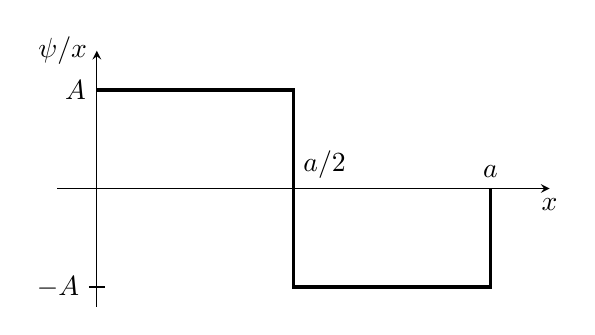
\begin{tikzpicture}
\draw[-stealth] (-0.5,0) -- (5.75,0)node[below]{$x$};
\draw[-stealth] (0,-1.5) -- (0,1.75)node[left]{$\dif\psi/\dif x$};
\draw[very thick](0,1.25) node[left]{$A$} -- (2.5,1.25) -- (2.5,-1.25) -- (5,-1.25) -- (5,0) node[above]{$a$};
\draw[] (-0.1,-1.25) node[left]{$-A$} -- (0.1,-1.25);
\draw[] (2.5,0) node[above right]{$a/2$};
\end{tikzpicture}
\caption{لامتناہی چکور کنواں میں تکونی تفاعل موج (شکل \حوالہ{شکل_تغیریت_لامتناہی_کنواں_تکونی_موج}) کا تفرق۔}
\label{شکل_تغیریت_لامتناہی_کنواں_تکونی_موج_تفرق}
\end{figure}


 اب سیڑھی تفاعل کا تفرق ایک Delta تفاعل ہے. سوال 2.24 ب دیکھے.
\[\frac{\dif^{2}{\psi}}{\dif{x^{2}}}=A\delta(x)-2A\delta(x-a/2)+A\delta(x-a)\]
لحاظہ درج ذیل ہوگا 
\begin{align*}
\langle H \rangle &= -\frac{\hbar^{2}A}{2m}\int[\delta(x)-2A\delta(x-a/2)+\delta(x-a)]\psi(x)\dif{x}\\
&= -\frac{\hbar^{2}A}{2m}[\psi(0)-2\psi(a/2)+\psi(a)]=\frac{\hbar^{2}A^{2}a}{2m}=\frac{12\hbar^{2}}{2ma^{2}}\\
\end{align*}
ٹھیک زمینی حال توانائی
\(E_{gs}=\frac{\pi^{2}\hbar^{2}}{2ma^{2}}\)
مساوات 2.27 ہے. لحاظہ یہ مثلہ کار آمد ہے. 
\(12>\pi^{2}\)\\

اصول تغيوریت انتہائی طاقتور اور استعمال کے نقطہ نظر سے شرمناک حد تک آسان ہے. کسی پیچده سالمہ کی زمینی حال توانائی جاننے کی خاطر ماہر کیمیا ایک ایسا پرکیا تفاعل موج منتخب کر کے٬ جس میں متعدد مقدار معلوم پائے جاتے ہو اور ان کی قیمتیں تبديل کرتے ہوئے
\( \langle H \rangle\)
کی کم سے کم ممکنہ قیمت تلاش کرے گا. اصل تفاعل موج کے ساتھ
\(\psi\) 
کی کوئی مشابہت نہ پائے جانے کی صورت میں بھی آپ کو
\( E_{gs}\)
 کی حیرت کن حد تک درست قیمت حاصل ہوگی۔ ظاہر ہے اگر آپ
\(\psi\) 
 کو حقیقی تفاعل کے زیادہ قریب منتخب کر پائے تو اتنا بہتر ہوگا. اس ترقيب کے ساتھ مسلہ یہ ہے کہ آپ کبھی بھی جان نہیں سکتے کہ آپ درست جواب کے کتنے قريب ہو. آپ صرف اتنا جانتے ہو کہ اصل جواب آپ کے نتیجہ سے كم ہوگا. مزید اس روپ میں یہ ترقيب صرف زمینی حال کے لیے کارآمد ہے. البتہ سوال 7.4 دیکھے.\\
سوال \\7.1
درجہ زیل مخفیہ کے لئے زمينی حال توانائی جاننے کی خاطر گاوسی پرکیا تفاعل\\:
مساوات 7.2 کی كم سے كم بالائی حد بندی تلاش كرے.\\
ا) خطی مخفیہ
\[V(x)=\alpha\abs{x}\]
ب) طاقت چار مخفیہ
\[V(x)=\alpha x^{4}\]
سوال \\7.2
 یک بودی ہارمونی مورتیش 
 \(E_{gs}\)
 کی بہترین حد بندی کو درج ذیل روپ کی پرکیا تفاعل موج
\[\psi(x)=\frac{A}{x^{2}+b^{2}}\]
استعمال کرکے تلاش كریں. جہاں معمول زنی سے تعائن ہوگا. جبکہ بھی قابل تبديل مقدار معلوم ہے.
 سوال 7.3 : \\
 ڈلتا تفاعل مخفیہ
\[-\alpha\delta(x)\]
کی
\(E_{gs}\) 
کی بہترین بالائی حد بندی کو دکونی پرکیا تفاعل مساوات 7.10. لیکن جس کا وسط مبده پر ہو استعمال کرکے تلاش كريں. یہاں a ایک قابل تبديل مقدار معلوم ہے.\\
سوال \\7.4
ا) اصول تغيوريت کے درج ذیل زمنی نتیجہ کو ثابت کریں. اگر
\(\langle \psi | \psi_{gs} \rangle =0\)
تب
\(\langle H \rangle \ge E_{fc}\)
ہوگا. جہاں پہلی ہیجان حال کی توانائی
 \(E_{fc}\)
 ہے. یوں اگر ہم کسی طرح ٹھیک زمینی حال کو امودی ایک پرکیا تفاعل تلاش كر سکے تب ہم پہلی ہیجان حال کی بالائی حد بندی جان سکتے ہیں. عموماً چونکہ ہم زمینی حال تفاعل
 \(\psi_{gs}\)
 کو نہیں جانتے ہے لحاظہ یہ کہنا مشکل ہوگا کہ ہمارا پرکی تفاعل 
 \(\psi\)
  اس کو امودی ہوگا. ہاں٬ اگر x کے لحاظ سے مخفی
 \(V(x)\)
   ایک جفت تفاعل ہو تب زمینی حال بھی جفت ہوگا. لحاظہ کوئی بھی تاگ پرکیا تفاعل خود بخود اس زمنی نتیجہ کے شرط پر پورا اترے گا.\\
ب) درج ذیل پرکیا تفاعل
\[\psi(x)=Axe^{-bx^{2}}\]
استعمال کرتے ہوئے یک بودی ہارمونی مورتیش کی پہلی ہیجان حال کا بہترین بالائی حد بندی تلاش كرے.\\
سوال 7.5    \\
ا) اصول تغيوریت استعمال کرکے ثابت کریں کہ رتبہ اول غير انحطاطی نظریہ استراب ہر صورت زمینی حال توانائی کی قیمت سے تجاوز کرے گا يا كم سے كم کبھی بھی اس سے كم قیمت نہیں دے گا.\\
ب) آپ جز آ جانتے ہوئے توقع کریں گے کہ زمینی حال کی دو رتبی تصحیح لاظمن منفی ہوگی. مساوات 6.15 کا معائنہ كرتے ہوئے تصدیق كريں کہ ایسا ہی ہوگا. \\

\حصہ{ہیلیم کا زمینی حال} 
ہیلیم جوہر  (شکل \حوالہ{شکل_تغیریت_ہیلیم_جوہر}) کے مرکزہ میں دو پروٹون اور دو نیوٹران جن کا یہاں کوئی کردار نہیں ہوگا پائے جاتے ہیں اور مرکزا کے گرد مدار میں دو الیکٹران حرکت کرتے ہیں۔
مہین ساخت اور باریک طزہی کو نظر انداز کرتے ہوئے اس نظام کا ہملٹھنی درج ذیل ہوگا 
\[H=-\frac{\hbar^{2}}{2m}(\nabla_{1}^{2}+\nabla_{2}^{2})-\frac{e^{2}}{4\pi\epsilon_{0}}\big (\frac{2}{r_{1}}+\frac{2}{r_{2}}-\frac{1}{\abs{\vec{r}_{1}-\vec{r}_{2}}}\big )\]

\begin{figure}
\centering
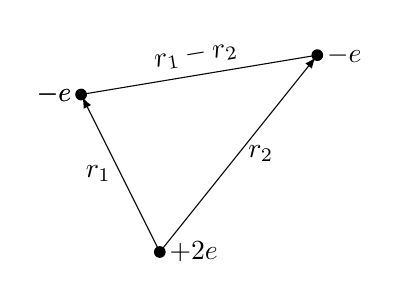
\begin{tikzpicture}
\draw[-latex,shorten >=1pt] (0,0) node[right]{$+2e$} node[circle, fill=black,inner sep=1.5pt]{} -- (-1,2) node[left]{$-e$} node[pos=0.5,left]{$\kvec{r}_1$};
\draw[] (-1,2) node[left]{$-e$} node[circle, fill=black,inner sep=1.5pt]{} -- (2,2.5) node[right]{$-e$} node[pos=0.5,above,sloped]{$\abs{\kvec{r}_1-\kvec{r}_2}$} node[circle, fill=black,inner sep=1.5pt]{};
\draw[-latex,shorten >=1pt] (0,0) -- (2,2.5) node[pos=0.5,right]{$\kvec{r}_2$};
\end{tikzpicture}
\caption{ہیلیم جوہر۔}
\label{شکل_تغیریت_ہیلیم_جوہر}
\end{figure}


ہم نے زمینی حال توانائی 
 \(E_{gs}\)
 کا حساب کرنا ہوگا ۔ طبی طور پر یہ دونوں الیکٹران اکھاڑنے کے لیے درکار توانائی کو ظاہر کرتا ہے۔ 
 \(E_{gs}\)
  جانتے ہوئے ہم ایک الیکٹران اکھاڑنے کے لیے درکار توانائی برداری عمل معلوم کر سکتے ہیں۔\\
سوال 7.6 دیکھیں\\ 
تجربہ گاہ میں ہیلیم کی زمینی حل توانائی کی قیمت کو انتہائی زیادہ درستگی تک پیمائش کیا گیا ہے ۔
\[E_{gs}=-78.975 \text{eV}\]
ہم نظریا سے اسی عدد کو حاصل کرنا چاہنگے۔ یہ تجسس کی بات ہے کہ ابھی تک اتنی سادہ اور اہم مسلے کا ٹھیک حل نہیں ڈھونڈا جا سکا ہے۔
مسلہ الیکٹران الیکٹران دفعہ 
\[V_{ee}=\frac{e^{2}}{4\pi\epsilon_{0}}\frac{1}{\abs{\vec{r}_{1}-\vec{r}_{2}}}\]
پیدا کرتا ہے۔ اس جز کو نظر انداز کرنے سے
 \(H \)
حایڑروجن ہملٹنیو میں الہدگا ہو جاتا ہے جہاں مرکزوی بار e کی بجائے
 \(2e\)
 ہوگا۔ اس کا ٹھیک ٹھیک حل حایڑروجن دفالاج ماج کا حاصل ظرب ہوگا ۔
\[\psi_{0}(\vec{r}_{1},\vec{r}_{2})\equiv \psi_{100}(\vec{r}_{1})\psi_{100}(\vec{r}_{2})=\frac{8}{\pi a^{3}e^{-2(r_{1}+r_{2})/a}}\]
اور توانائی
 \(8E_{1}=-109\text{eV}\)
 الیکٹران وولٹ 
مساوات 5.31 ہوگی ۔ یہ قیمت
 \(-79\text{eV}\) 
 الیکٹران وولٹ سے بہت دور ہے ۔ تاہم یہ صرف آغاز ہے ۔ ہم فایے ناٹ کو بھر کیا افعال معاج لیتے ہوئے 
 \(E_{gs}\)
 کی بہتر تخمیم کو اصول تغیریت سے حاصل کرتے ہیں چونکہ یہ زیادہ تر ہملٹھنی کا امتیازی دفعال ہے لہذا یہ خصوصی طور پر بہتر انتخاب ہے۔
\[H\psi_{0}=(8E_{1}+V_{ee})\psi_{0}\]
یوں درج ذیل ہوگا۔ 
\[\langle H \rangle=8E_{1}+\langle V_{ee}\rangle\]
جہاں درج ذیل ہے 
\[\langle V_{ee}\rangle=\big(\frac{e^{2}}{4\pi\epsilon_{0}}\big )\big (\frac{8}{\pi a^{3}}\big )^{2}\int \frac{e^{-4(r_{1}+r_{2})/a}}{\abs{\vec{r}_{1}-\vec{r}_{2}}}d^{3}\vec{r}_{1}d^{3}\vec{r}_{2}\]

\begin{figure}
\centering
\begin{tikzpicture}[x={(-0.5cm,-0.5cm)}, y={(1cm,0cm)}, z={(0cm,1cm)}]
\pgfmathsetmacro{\p}{atan(2/0.5)}
\pgfmathsetmacro{\t}{acos(2.5/sqrt(0.5^2+2^2+2.5^2))}
\draw[-stealth] (0,0,0) -- (1.5,0,0) node[left]{$x_2$};
\draw[-stealth] (0,0,0) -- (0,3,0) node[below]{$y_2$};
\draw[-stealth] (0,0,0) -- (0,0,3) node[left]{$z_2$};
\draw[very thick, -latex,shorten >=1pt] (0,0,0) node[circle, fill=black,inner sep=1.5pt]{} -- (0,0,2) node[pos=0.75,left]{$\kvec{r}_1$};
\draw[very thick] (0,0,2) node[circle, fill=black,inner sep=1.5pt]{} -- (0.5, 2, 2.5) node[pos=0.5,above,sloped]{$\abs{\kvec{r}_1-\kvec{r}_2}$} node[circle, fill=black,inner sep=1.5pt]{};
\draw[very thick, -latex,shorten >=1pt] (0,0,0) -- (0.5,2,2.5) node[pos=0.5,right]{$\kvec{r}_2$};
\draw[dashed] (0,0,0) -- (0.5,2,0) -- (0.5,2,2.5);
\begin{scope}[canvas is xy plane at z=0]
\draw[-stealth] ([shift=(0:0.75)]0,0,0) arc (0:75:0.75)node[pos=0.5,below right]{$\phi_2$};
\end{scope}
\draw[-stealth,domain=0:\t] plot ({1*sin(\x)*cos(\p)},{1*sin(\x)*sin(\p)},{cos(\x)});
\draw(0,0.4,0.8)node[above]{$\theta_2$};
\end{tikzpicture}
\caption{محدد کا انتخاب برائے \عددی{\kvec{r}_2} تکمل (مساوات \حوالہء{7.20})۔}
\label{شکل_تغیریت_محدد_انتخاب_رداس_دوم_تکمل}
\end{figure}


میں 
\(r_{2}\)
 تکمل کو پہلے حل کرتا ہوں ۔یوں
 \(r_{1}\)
کو مستقل تصور کیا جائے گا ۔\\
ہم 
\(r_{2}\)
کے محددی نظام کو یوں رکھتے ہیں کہ اس کا قطبی محور
 \(r_{1}\)
پر پایا جاتا ہو (شکل \حوالہ{شکل_تغیریت_محدد_انتخاب_رداس_دوم_تکمل})۔
قانون کوسائن کے تحت 
\[\abs{\vec{r}_{1}-\vec{r}_{2}}=\sqrt{r_{1}^{2}+r_{2}^{2}-2r_{1}r_{2}\cos{\theta_{2}}}\]
لحاضہ درج ذیل ہوگا \\
\[I_{2}\equiv\int\frac{e^{-4r^{2}/a}}{\abs{\vec{r}_{1}-\vec{r}_{2}}}d^{3}r_{2}=\int\frac{e^{-4r^{2}/a}}{\sqrt{r_{1}^{2}+r_{2}^{2}-2r_{1}r_{2}\cos{\theta_{2}}}}r_{2}^{2}\sin{\theta_{2}}dr_{2}d\theta_{2}d\phi_{2}\]
متغیر 
\(\phi_{2}\)
کا (نہایت آسان) تکمل 
\(2\pi\)
 دے گا۔\\
متغیر 
\(\theta_{2}\)
 کا تکمل درج ذیل ہوگا
\begin{align*}
\int_{0}^{\pi}\frac{\sin{\theta_{2}}}{\sqrt{r_{1}^{2}+r_{2}^{2}-2r_{1}r_{2}\cos{\theta_{2}}}}\dif{\theta_{2}}=\frac{\sqrt{r_{1}^{2}+r_{2}^{2}-2r_{1}r_{2}\cos{\theta_{2}}}}{r_{1}r_{2}}|_{0}^{\pi}
\end{align*}
\begin{align*}
&=\frac{1}{r_{1}r_{2}}(\sqrt{r_{1}^{2}+r_{2}^{2}+2r_{1}r_{2}}-\sqrt{r_{1}^{2}+r_{2}^{2}-2r_{1}r_{2}})\\
&=\frac{1}{r_{1}r_{2}}[(r_{1}+r_{2})-\abs{r_{1}-r_{2}}]=\begin{cases}
2/r_{1} & r_{2}<r_{1}\\
2/r_{2}&r_{2}>r_{1}\\
\end{cases}\\
\end{align*}
یوں درج ذیل ہوگا 
\begin{align*}
I_{2}&=4\pi(\frac{1}{r_{1}}\int_{0}^{r_{1}}e^{-4r_{2}/a}r_{2}^{2}dr_{2}+\int_{r_{1}}^{\infty}e^{-4r_{2}/a}r_{2}dr_{2})\\
&=\frac{\pi a^{3}}{8r_{1}}[1-(1+\frac{2r_{1}}{a})e^{-4r_{1}/a}]\\
\end{align*}
اس طرح 
\(\langle V_{ee} \rangle \)
درج ذیل ہوگا ۔
\[(\frac{e^{2}}{4\pi\epsilon_{0}})(\frac{8}{\pi a^{3}})\int[1-(1+\frac{2r_{1}}{a})e^{-4r_{1}/a}]e^{-4r_{1}/a}r_{1}\sin{\theta_{1}}dr_{1}d\theta_{1}d\phi_{1}\]
ظوایائی تکملات 
\(4\pi\)
دینگے جبکہ 
\(r_{1}\)
 کا تکمل درج ذیل ہوگا
\[\int_{0}^{\infty}[re^{-4r/a}-(r+\frac{2r^{2}}{a})e^{-8r/a}]dr=\frac{5a^{2}}{128}\]
آخر میں اس طرح درج ذیل ہوگا 
\[\langle V_{ee} \rangle\frac{5}{4a}(\frac{e^{2}}{4\pi\epsilon_{0}}=-\frac{5}{2}E_{1}=34\text{eV}\]
جس کی بنا درج ذیل ہوگا 
\[\langle H \rangle =-109 \text{eV}+34 \text{eV}=-75\text{eV}\]
یہ جواب زیادہ برا نہیں ہے۔
یاد رہے کہ تجرباتی قیمت 79- الیکٹران وولٹ ہے۔\\
تاہم ہم اس سے بھی بہتر کر سکتے ہیں۔
ہم
\(\psi_{0}\)
جو دو الیکٹرانوں کو یوں تصور کرتا ہے جیسا ایک دوسرے پر اصر انداز نہیں ہوتے ہیں۔
سے بہتر زیادہ حقیقت پسندانہ پھر کیا دفعال کا سوچ سکتے ہیں۔
ایک الیکٹران کا دوسرے الیکٹران پر اصر کو مکمل طور پر نظر انداز کرنے کی بجائے ہم کہتے ہیں کہ ایک الیکٹران قواسطن منفی بار کی بطل کی طرح ہوگا جو مرکزا کو جزوی طور پر سپر کرتا ہے جس کی بنا دوسرے الیکٹران کو موثر مرکزوی بار z کی قیمت 2 سے کچھ کم نظر آئے گی۔ اس سے ہمیں خیال آتا ہے کہ ہم درج ذیل روپ کا برقی دفعال استعمال کریں۔
\[\psi_{1}(r_{1},r_{2})=\frac{Z^{3}}{\pi a^{3}e^{-Z(r_{1}+r_{2})/a}}\]
ہم z کو تخیریت کا مقدار معلوم تصور کر کہ اس کی وہ تمام قیمت منتخب کر کے جس سے H کی کم سے کم قیمت حاصل ہو ۔
دیہان رہے کہ فضول تغیریت کی ترقیب کبھی بھی ہمیلٹنی کو تبدیل نہیں کرتا ہے ۔
ہیلیم کا ہمیلٹنی اب بھی مساوات 
مساوات 7.14
دیگی البتہ
تصور میں ہمیلٹنی کی تخمیمی قیمت کے بارے میں سوچ کے بہتر بلکیا دفعال معاج حاصل کیا جا سکتا ہے ۔
یہ دفعال معاج اس غیر مضطرب ہمیلٹنی جو الیکٹران کی دفعہ کو نظر انداز کرتا ہو جس میں جز coulumb میں دو کی جگہ z پایا جاتا ہو کا امتیازی حال ہوگا۔
اس کو ذہن میں رکھتے ہوئے ہم 7.14 H کو روپ میں لکھتے ہیں 
\[-\frac{\hbar^{2}}{2m}(\nabla_{1}^{2}+\nabla_{2}^{2})-\frac{e^{2}}{4\pi\epsilon_{0}}(\frac{Z}{r_{1}}+\frac{Z}{r_{2}})+\frac{e^{2}}{4\pi\epsilon_{0}}(\frac{(Z-2)}{r_{1}}+\frac{(Z-2)}{r_{2}}+\frac{1}{\abs{\vec{r_{1}}-\vec{r}_{2}}})\]
ظاہر ہے کہ H کی تحقیقاتی قیمت درج ذیل ہوگی 
\[\langle H \rangle = 2Z^{2}E_{1}+2(Z-2)(\frac{e^{2}}{4\pi\epsilon_{0}})\langle \frac{1}{r}\rangle + \langle V_{ee} \rangle \]
یہاں
\(\langle 1/r \rangle \) 
سی مراد ایک ظرہ ہائڈروجن زمینی حال سائے 100 جس میں مرکزوی بار 
Z
 ہو میں
\(1/r\)
کی تحقیقاتی قیمت ہے ۔\\
یوں مساوات 6.55 کے تحت درج ذیل ہوگا 
\[\langle \frac{1}{r} \rangle = \frac{Z}{a}\]
یہاں بھی vee کی توقیاتی قیمت وہی ہوگی جو پہلے تھی۔
مساوات 7.65لیکن اب ہم z =2 کی بجائے اختیار z استعمال کریں گے لہذا ہم a کو 
\(2/Z\)
 سے ظرب کرتے ہیں 
 \[\langle V_{ee} \rangle =\frac{5Z}{8a}(\frac{e^{2}}{4\pi\epsilon_{0}})=\frac{5Z}{4}E_{1}\]
 ۔ان تمام کو اکٹھے کر کہ درج ذیل حاصل ہوگا 
 \[\langle H \langle =[2Z^{2}-4Z(Z-2)-(5/4)Z]E_{1}=[-2Z^{2}+(27/4)Z]E_{1}\]
اصول تغیریت کے تحت z کی کسی قیمت کے لیے بھی یہ مقدار 
\(E_{gs}\)
سے تجاوظ کرے گی ۔\\
بالائی حد بندی کی کم سے کم قیمت وہاں پائی جانے گی جب
 \(\langle H \rangle \)
 کی قیمت کن سے کم ہو۔\\
\[\frac{d}{dZ}\langle H \rangle =[-4Z+(27/4)]E_{1}=0\]
جس سے درج ذیل حاصل ہوگا۔
\[Z=\frac{27}{16}=1.69\]
یہ ایک معقول نتیجہ نظر آتا ہے جو کہتا ہے دوسرا الیکٹران مرکزا کو سپر کرتا ہے جس کی بنا اس کی موثر بار 2 کی بجائے 1.69 نظر آتی ہے ۔اس قیمت کو z میں پر کر کہ درج ذیل حاصل ہوگا ۔\\
\[\langle H \rangle =\frac{1}{2}(\frac{3}{2})^{6}E_{1}=-77.5\text{eV}\]
قبلے تقدیر معا معلوم کی تعداد بڑھا کر زیادہ پیچیدہ پرکیا دفعالات معاج لے کر ہیلیم کی زمینی حال توانائی کو اسی ترقیب سے انتہائی زیادہ درستگی تک حاصل کیا گیا ہے ہم ٹھیک جواب کے دو فیسٹ قریب ہیں لحاضہ اس کو یہیں پر چھوڑتے ہیں ۔\\
سوال 
7.6\\
ہیلیم کی زمینی حال توانائی 
\(E_{gs}=-79\text{eV}\)
 لیتے ہوئے توانائی بار داری حمل صرف ایک الیکٹران اکھاڑنے کے لیے درکار توانائی کا حساب کریں ۔\\
اشارہ پہلے ہیلیم بارداریا
 \(He^{+}\)
 جس کے مرکزا کے گرد صرف ایک الیکٹران مدار میں حرکت کرتا ہے کی زمینی حال توانائی تلاش کریں ۔\\
اس کے بعد دونوں توانائیوں کا فرق لیں 
سوال 7۔7
\\
اس حصہ میں ملتمل ترقیبات کا اتلاک
 \(H^{-}\)
 اور
 \(Li^{+}\)
 بارداریا جن میں ہلیم کی طرح دو الیکٹران پائے جاتے ہیں اور جن کی مرکزوی بار بالترتیب z=1 , z=3 ہیں کریں ۔\\
باریک باریک ایک ایک بارداریا کے لیے کا موثر جزوی سپر شدا مرکزوی بار تلاش کر کہ 
\(E_{gs}\)
 کی بہترین بالائی حقبندی متعین کریں ۔\\
 بارداریا
 \(\text{H}^{-}\)
 کی صورت میں آپ دیکھیں گے کہ 
 \(\langle H \rangle > -13.6\text{eV}\) 
 ہوگا جس کے تحت کوئی مقید حآل نہیں ہوگا ۔
توانائی کی نقطہ نظر سے زیادہ بہتر صورتحال یہ ہوگی کہ الیکٹران درست ہو کر پیچھے مدرل حاڈروجن جوہر چھوڑے۔ یہ زیادہ حیرانگی کی بات نہیں ہے چونکہ ہیلیم کے لحاظ سے یہاں الیکٹران اور مرکزا کے بیچ قوت کشش کم ہے ۔ جبکہ الیکٹرانوں کے بیچ قوت دفعہ زیادہ ہے۔
جو اس جوہر کے توڑے گا حقیقت میں یہ نتیجہ درست نہیں ہے ۔ زیادہ نفیس برکیا دفعال معاج ساتھ 
7.18
دیکھیں 
منتخب کر کے دکھایا جا سکتا ہے کہ 
\(E_{gs}<-13.6\text{eV}\)
ہوگا لحاضہ مقید حآل موجود ہوگا ۔
البتہ یہ بمشکل مقید ہوگا اور کوئی حجانی مقید حالات نہیں پائے جاتے ہیں یوں
\(\text{ H}^{-}\)
 کا غیر مسلسل طیف نہیں پایا جاتا ہے ۔
تمام عبور ازتمراریا کو اور ازتمراریا سے ہوں گے اسی لیے ان کا متالیا تجربہ گاہ میں کرنا دشوار ثابت ہوتا ہے اگرچہ سورج کی سطح پر ان کی کثیر تعداد پائی جاتی ہے ۔\\
\
\حصہ{ہائیڈروجن سالمہ بار داریہ}\شناخت{حصہ_تغیری_اصول_ہائیڈروجن_بارداریہ}
اصول تغیریت کی ایک اور پلاسی کی استعمال۔ ہائیڈروجن سالمہ بار داریہ
\(\text{ H}_{2}^{+}\)
 کا معائنہ ہے۔ ہائیڈروجن سالمہ بار داریہ دو پروٹان کی کولمب میدان میں ایک الیکڑان پر مشتمل ہے (شکل \حوالہ{شکل_تغیریت_ہائیڈروجن_سالمہ_بارداریہ})۔ 
میں فی الوقت فرض کرتا ہوں کہ دونوں پروٹان ساکن ہیں اور ان کے بیچ فاصلہ R ہے۔ اگرچہ اس حساب کا ایک دلچسپ ذیلی نتیجہ R کی اصل قیمت ہوگی۔ ہمیٹنی درجہ ذیل ہوگا۔
 \[H=-\frac{\hbar^{2}}{2m}\nabla^{2}-\frac{e^{2}}{4\pi\epsilon_{0}}(\frac{1}{r_{1}}+\frac{1}{r_{2}}\]
جہاں
\( r_{1}\) 
اور 
\(r_{2}\) 
الیکڑان سے متعلقہ پروٹان تک فاصلہ ہے۔ ہمیشہ کی طرح ہم کوشش کریں گے کہ ایک ایسا پھر کی طفال موج کا انتخاب کریں جس کو استعمال کرتے ہوئے زمینی حال توانائی کی حد بندی اصول تغیریت سے حاصل ہو۔ در حقیقت ہم صرف اتنا جاننا چاہتے ہیں کہ آیا اس نظام میں بند پیدا ہوگا یعنی آیا ایک مادل ہائیڈروجن جوہر اور ایک آزاد پروٹان سے کیا اس نظام کی توانائی کم ہوگی۔ آگر ہماری پھر کی طفال موج دکھائے کہ ایک مکید حال پایا جاتا ہے۔ اس سے زیادہ بہتر پھر کی طفال اس بند کو مزید طاقتور بنائے گا۔
\begin{figure}
\centering
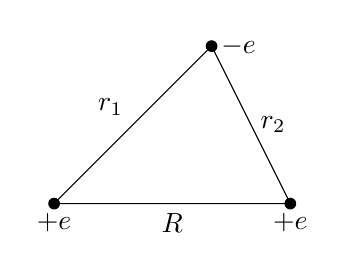
\begin{tikzpicture}
\draw[] (0,0) node[below]{$+e$} node[circle, fill=black,inner sep=1.5pt]{} -- (3,0) node[pos=0.5, below]{$R$} node[below]{$+e$} node[circle, fill=black,inner sep=1.5pt]{} -- (2,2) node[pos=0.5, right]{$r_2$} node[right]{$-e$} node[circle, fill=black,inner sep=1.5pt]{} -- (0,0) node[pos=0.5, above left]{$r_1$};
\end{tikzpicture}
\caption{ہائیڈروجن سالمہ بارداریہ، \عددی{\ce{H}_2^+}}
\label{شکل_تغیریت_ہائیڈروجن_سالمہ_بارداریہ}
\end{figure}


 پھر کی طفال موج تیار کرنے کی خاطر فرض کریں زمینی حال مہوار 4.80
\[\psi_{0}(r)=\frac{1}{\sqrt{\pi a^{3}}}e^{-r/a}\]
 میں ایک ہائیڈروجن جوہر کے قریب لا متناہی دوسرا پروٹان قریب لا کر فاصلہ R پر رکھ کر بار داریہ پیدا کیا جاتا ہے۔ اگر رداس بوہر سے r کافی بڑا ہو تب الیکڑان کی طفال موج غالبا زیادہ تبدیل نہیں ہو گا۔ تاہم ہمیں دونوں پروٹانوں کو ایک نظر سے دیکھنا ہوگا۔ لہذا کسی ایک کے ساتھ الیکڑان کی وابستگی کا احتمال ایک دوسرے جیسا ہوگا۔ اس سے ہمیں خیال آتا ہے کہ ہم درجہ ذیل روپ کے پھر کی طفال 
 \[\psi=A[\psi_{0}(r_{1})+\psi_{0}(r_{2})]\]
 پر غور کریں\\
۔ ماہر کوانٹم کیمیا اس ترکیب کو جوہری مدارچوں کا خطی جوڑ کہتے ہیں۔ \\
سب سے پہلا کام پھر کی طفال کی معمول زنی ہے۔
 \[1=\int\abs{\psi}^{2}d^{3}r=\abs{A}^{2}\big [\int \abs{\psi_{0}(r_{1})}^{2}d^{3}r+\int \abs{\psi_{0}(r_{2})}^{2}d^{3}r+2\int\psi_{0}(r_{1})\psi_{0}(r_{2})d^{3}r\big ]\]
پہلے دو تکلملات کا نتیجہ ایک ہے۔ چونکہ 
\(\psi_{0}\)
خود معمول شدہ ہے۔ تیسرا زیادہ پیچیدہ ہے۔ درجہ ذیل فرض کریں۔\\
 \[I\equiv\langle \psi_{0}(r_{1})|\psi_{0}(r_{2})\rangle=\frac{1}{\pi a^{3}}\int e^{-(r_{1}+r_{2})/a}d^{3}r\]
ایسا معتدی نظام کھڑا کریں جس کہ نقطہ پر پروٹان 1 پایا جاتا ہو جبکہ Z مہور پر فاصلہ R پر پروٹان 2 پایا جاتا ہو (شکل \حوالہ{شکل_تغیریت_محدد_قدار_آئے})۔ یوں درجہ ذیل ہوگا۔ \\
\[r_{1}=r \quad r_{2}=\sqrt{r^{2}+R^{2}-2rR\cos{\theta}}\]
%
\begin{figure}
\centering
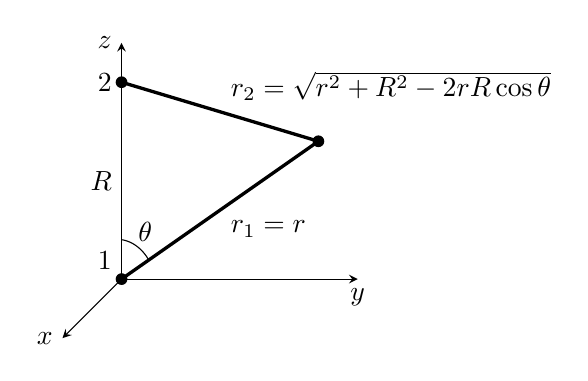
\begin{tikzpicture}[x={(-0.5cm,-0.5cm)}, y={(1cm,0cm)}, z={(0cm,1cm)}]
\pgfmathsetmacro{\p}{atan(2/0.5)}
\pgfmathsetmacro{\t}{acos(2/sqrt(0.5^2+2.75^2+2^2))}
\draw[-stealth] (0,0,0) -- (1.5,0,0) node[left]{$x$};
\draw[-stealth] (0,0,0) -- (0,3,0) node[below]{$y$};
\draw[-stealth] (0,0,0) -- (0,0,3) node[left]{$z$};
\draw[] (0,0,0) node[above left]{$1$} node[circle, fill=black,inner sep=1.5pt]{} -- (0,0,2.5) node[left]{$2$} node[pos=0.5,left]{$R$};
\draw[very thick] (0,0,2.5) node[circle, fill=black,inner sep=1.5pt]{} -- (0.5, 2.75, 2) node[pos=0.5,above right]{$r_2=\sqrt{r^2 + R^2 -2rR\cos \theta}$} node[circle, fill=black,inner sep=1.5pt]{};
\draw[very thick] (0,0,0) -- (0.5,2.75,2) node[pos=0.5,below right]{$r_1=r$};
\draw[domain=0:\t] plot ({0.5*sin(\x)*cos(\p)},{0.5*sin(\x)*sin(\p)},{0.5*cos(\x)});
\draw(0,0.3,0.6)node[]{$\theta$};
\end{tikzpicture}
\caption{مقدار \عددی{I} کے حساب کی خاطر محدد (مساوات \حوالہء{7.39})۔}
\label{شکل_تغیریت_محدد_قدار_آئے}
\end{figure}

%
لہذا درجہ ہوگا \\
\[I=\frac{1}{\pi a^{3}}\int e^{-r/a}e^{-\sqrt{r^{2}+R^{2}-2rR\cos{\theta/a}}}r^{2}\sin{\theta}drd\theta d\phi\]
متغیر 
\(\phi\)
 کا (نہایت آسان) تکمل 
 \(2\pi\)
 دے گا۔ متغیر 
 \(\theta\)
  کا تکمل حل کرنے کی خاطر درجہ ذیل لیں۔\\
\[y\equiv\sqrt{r^{2}+R^{2}-2rR\cos{\theta}}\]
لہذا 
\[d(y^{2})=2ydy=2rR\sin{\theta}d\theta\]
ہوگا۔ تب درجہ ذیل ہوگا۔
\[\int_{0}^{\pi}e^{-\sqrt{r^{2}+R^{2}-2rR\cos{\theta/a}}}\sin{\theta}d\theta=\frac{1}{rR}\int_{\abs{r-R}}^{r+R}e^{-y/a}ydy=-\frac{-a}{rR}[e^{-(r+R)/a}(r+R+a)-e^{-\abs{r-R}/a}(\abs{r-R}+a)]\]
اب تکمل r با آسانی حل ہوگا۔ 
\[I=\frac{2}{a^{2}R}[-e^{-R/a}\int_{0}^{\infty}(r+R+a)e^{-2r/a}rdr+e^{-R/a}\int_{0}^{R}(R-r+a)rdr+e^{R/a}\int_{R}^{\infty}(r-R+a)e^{-2r/a}rdr]\]
ان تکملات کی قیمتیں حاصل کرنے کے بعد کچھ الجبرائی تصحیل کے بعد درجہ ذیل حاصل ہوگا۔
\[I=e^{-R/a}\big[1+(\frac{R}{a}+\frac{1}{3}(\frac{R}{a})^{2}\big]\]
ےھاں  ٰI کو مکمل ڈمب کہتے ہیں جو۔
\(\psi_{0}(r_{1})\)
 کا۔
 \(\psi_{0}(r_{2}\)
 پر چڑھنے کی مقدار کی پیمائش ہے۔ دیہان رہے کہ 
 \(R\rightarrow 0\)
 کی صورت میں یہ ایک پہنجتا ہے۔جبکہ 
 \(R\rightarrow \infty\)
  کی صورت میں یہ صفر کو پہنجتا ہے۔ تکمل ڈنب i میں جز زربی معمول زنی مساوات 7.38 درجہ ذیل ہوگا ۔\\
\[\abs{A}^{2}=\frac{1}{2(l+1)}\]
اس کے بعد ہمیں پھر کی حال 
\(\psi\)
 میں H کی توقعاتی قیمت کا حساب کرنا ہوگا۔ درجہ ذیل ۔
 \[\big(-\frac{\hbar^{2}}{2m}\nabla^{2}-\frac{e^{2}}{4\pi\epsilon_{0}}\frac{1}{e_{1}}\big)\psi_{0}(r_{1})=E_{1}\psi_{0}(r_{1})\]
 جہاں 
 \(E_{1}=-13.6\text{eV}\)
 جوہری ہائیڈروجن کی زمینی حال توانائی ہے اور r1 کی جگہ r2 کے لئے بھی یہی کچھ کے بنا درجہ ذیل ہوگا ۔
\begin{align*}
H\psi&=A\big[-\frac{\hbar^{2}}{2m}\nabla^{2}-\frac{e^{2}}{4\pi\epsilon_{0}}\big(\frac{1}{r_{1}}+\frac{1}{r_{2}}\big)\big][\psi_{0}(r_{1})+\psi_{0}(r_{2})]\\
&=E_{1}\psi-A(\frac{e^{2}}{4\pi\epsilon_{0}}\big[\frac{1}{r^{2}}\psi_{0}(r_{1})+\frac{1}{r_{1}}\psi_{0}(r_{2})\big]
\end{align*}
یوں H کی توقعاتی قیمت درجہ ذیل ہوگی۔
\[\langle H \rangle =E_{1}-2\abs{A}^{2}\big(\frac{e^{2}}{4\pi\epsilon_{0}}\big)\big[\langle \psi_{0}(r_{1})\abs{\frac{1}{r_{2}}}\psi_{0}(r_{1})\rangle +\langle \psi_{0}(r_{1})\abs{\frac{1}{r_{1}}}\psi_{0}(r_{2})\rangle\big]\]
میں آپ کے لئے باقی دو مقدار جو بلا واسطہ تکمل 
\[D\equiv a\langle \psi_{0}(r_{1})\abs{\frac{1}{r_{2}}}\psi_{0}(r_{1})\rangle\]
اور
مبادلہ تکمل 
\[X\equiv a\langle\psi_{0}(r_{1})\abs{\frac{1}{r_{1}}}\psi_{0}(r_{2})\rangle\]
کہلاتا ہے۔ حل کرنے کے لئے چھورتا ہوں۔ بلا واسطہ تکمل کا نتیجہ درجہ ذیل 
\[D=\frac{a}{R}-\big(1+\frac{a}{R}\big)e^{-2R/a}\]
اور مبادلہ تکمل کا نتیجہ درجہ ذیل ہے ۔ 
\[X=\big(1+\frac{R}{a}\big)e^{-R/a}\]
ان تمام نتائج کو اکھٹے کرتے ہوئے اور یاد رکھتے ہوئے مساوات 4.70 اور 4.72 کہ 
\(E_{1}=-(e^{2}/4\pi\epsilon_{0})(1/2a)\)
ہے ۔ ہم درجہ ذیل آخذ کرتے ہیں۔
\[\langle H \rangle =\big[a+2\frac{(D+X)}{(1+L)}\big]E_{1}\]
اصول تغیریت کے تحت زمینی حال توانائی 
\(\langle H \rangle\)
 سے کم گی۔ یقینا یہ صرف الیکڑان کی توانائی ہے۔ اس کے ساتھ پروٹان پروٹان دفع سے وابستہ مخفی توانائی بھی پائ جائے گی۔.
\[V_{pp}+\frac{e^{2}}{4\pi\epsilon_{0}}\frac{1}{R}=-\frac{2a}{R}E_{1}\]
یوں نظام کی کل توانائی مائنس
\(E_{1}\)
 کی اکائیوں میں 
 \(x\equiv R/a\)
 کا طفال لکھتے ہوئے درجہ ذیل سے کم ہو گا۔
 \[F(x)=-1+\frac{2}{X}\big\{\frac{(1-(2/3)x^{2})e^{-x}+(1+x)e^{-2x}}{1+(1+x+(1/3)x^{2})e^{-x}}\big\}\]
اس طفال کو شکل  \حوالہ{شکل_تغیریت_مقید_حال} میں ترسیم کیا گیا ہے۔ اس ترسیم کا کچھ حصہ منفی ایک سے نیچے ہے۔ جہاں معدل جوہر جمع ایک آزاد پروٹان کی توانائی مائنس 13.6الیکڑان وولٹ سے توانائی کم ہے۔ لہذا اس نظام میں بند پیدا ہوگا۔ یہ ایک شریک گرفتی بند ہوگا، جہاں دونوں پروٹانوں کا الیکڑان میں ایک دوسرے کے برابر حصہ ہوگا۔ پروٹانوں کے بیچ توازنی فاصلہ تقریبا 2.4 رداس بوہر یعنی 1.3 اینگسڑروم ہے۔ جس کی تجرباتی قیمت 1.06 اینگسڑروم ہے۔ توانائی بندش کی حساب سے حاصل قیمت 1.8 الیکڑان وولٹ جبکہ پیمائشی قیمت 2.8 الیکڑان وولٹ ہے۔ چونکہ اصول تغیریت ہر صورت زمینی حال توانائی سے تجاوز کرتا ہے لہذا یہ بندش کی طاقت کی قیمت کم دے گا۔ بہرحال اس کی فکر نہ کریں۔ یہاں اہم نقطہ یہ ہےکہ بندش پایا جاتا ہے۔ ایک بہتر تغیراتی طفال اس مخفیہ کو مزید گہرا کرے گا۔ 
\begin{figure}
\centering
\begin{tikzpicture}[declare function={fa(\x)=(1-2/3*\x^2)*e^(-\x); fb(\x)=(1+\x)*e^(-2*\x); fc(\x)=1+(1+\x+1/3*\x^2)*e^(-\x); f(\x)=-1+2*(fa(\x)+fb(\x))/(\x*fc(\x));}]
\begin{axis}[axis lines=middle,axis x line shift=1,xlabel={$x$},ylabel={$F(x)$}, xtick={1,2,2.25,3,4,5,6}, xticklabels={$1$,$2$,,$3$,$4$,$5$,$6$}, ytick={-1.2,-1,-0.5,0}, ylabel style={at={(current axis.above origin)},anchor=east},,enlargelimits,ymax=0,ymin=-1.3]
\addplot [thick,domain=0.7:6,smooth] {f(x)};
\addplot[thick] coordinates {(2.25,-1.025)(2.25,-0.975)};
\addplot[] coordinates{(2.25,-1)} node[pin={45:{توازن}}]{};
\end{axis}
\end{tikzpicture}
\caption{تفاعل \عددی{F(x)} (مساوات \حوالہء{7.51}) کی ترسیم مقید حال کی موجودگی دکھاتی ہے (بوہر رداس کی اکائیوں میں \عددی{x} دو پروٹانوں کے بیچ فاصلہ ہے)۔ }
\label{شکل_تغیریت_مقید_حال}
\end{figure}


سوال 
7.8\\
بلاواسطہ تکمل D اور مبادلہ تکمل X مساوات 7.45 اور 7.46 کی قیمتیں تلاش کریں۔ اپنے جوابات کا موازنہ مساوات 7.47 اور 7.48 کے ساتھ کریں۔ \\
سوال 
7.9\\
فرض کریں ہم نے پھرکی طفال موج مساوات 7.37 میں منفی علامت استعمال کی ہوتی ۔
\[\psi=A[\psi_{0}(r_{1})-\psi_{0}(r_{2})]\]
کوئی نیا تکمل حل کیے بغیر مساوات 7.51 کا مماسل
\( F(x)\) 
معلوم کر کے ترسیم کریں۔ دکھائیں کہ ایسی صورت میں بند پیدا نہیں ہوگا۔ چونکہ اصول تغیریت صرف بالائی حد بندی دیتا ہے لہذا اس سے یہ ثابت نہیں ہوگا کہ ایسے حال میں بند نہیں پایا جائے گا۔ تاہم اس سے زیادہ امید بھی نہیں کرنی چاہیئے۔ تبصرہ در حقیقت درجہ ذیل روپ کا کوئی طفال 
\[\psi=A[\psi_{0}(r_{1})+e^{i\phi}\psi_{0}(r_{2})]\]
کی ایک خاصیت یہ ہے کہ الیکڑان دونوں پروٹان کے ساتھ برابر کا وابستگی رکھتا ہے۔ تاہم چونکہ باہمی ادل بدل 
\(P: r_{1}\leftrightarrow r_{2}\)
کی صورت میں ہملٹنی مساوات 7.35 غیر متغیر ہے۔ لہذا اس کے امتیازی طفالات کو بیک وقت P کے امتیازی طفالات چنا جا سکتا ہے۔ امتیازی قدر
\(+1\)
کے ساتھ مثبت علامت۔ مساوات 7.37 اور امتیازی قدر منفی 1 کے ساتھ منفی علامت مساوات 7.52 ہوگا۔ زیادہ عمومی صورت مساوات 7.53 کا استعمال مزید فائدہ نہیں دے گا۔ اگرچہ آپ چاہیں تو اسے استعمال کر کے دیکھ سکتے ہیں۔\\
سوال 
7.10\\
نقطہ توازن پر
\( F(x)\)
 کی دوہرا تفرق سے ہائیڈروجن سالمہ بار داریہ حصہ 2.3 میں دونوں پروٹانوں کی ارتعاش کی قدرتی تعدد اومیگہ کی انداز قیمت تلاش کی جا سکتی ہے۔ اگر اس موردیش کی زمینی حال توانائی 
 \(\hbar\omega/2\)
 نظام کی بندشی توانائی سے زیادہ ہو تب نظام بکھر کر ٹوٹ جائے گا ۔ دکھائیں کہ حقیقت میں موردیش توانائی اتنی کم ہے کہ ایسا کبھی بھی نہیں ہوگا۔ ساتھ ہی مکید لرزشی سطحوں کی انداز تعداد دریافت کریں۔ تبصرہ 
آپ دہلیلی طور پر کم سے کم نقطہ یا اس نقطہ پر دوہرا تفرق حاصل نہیں کر پائیں گے۔ اعدادی طریقہ یا کمپیوٹر کی مدد سے ایسا کیجئے گا۔\\
سوال 
7.11\\
الف ) درج ذیل روپ کا برکی تفال موج
\[\psi(x)=\begin{cases}
A\cos{(\pi x/a)} & (-a/2<x<a/2)\\
0\\
\end{cases}\]
دیگر صورت
اس کا استعمال کرتے ہوئے یک بودی ہارمونی مرتعش کی زمینی حال توانائی کی حدبندی تلاش کریں . a کی بہترین قیمت کیا ہوگی . H کمتر کا معازنہ ٹھیک توانائی سے کریں .
تبصره : بر کی تفال میں
\(\pm a/2\)
پر ایک بل پایا جاتا ہے ایک غیر استمراری تفرک کیا آپ تو اس سے نمٹنا ہوگا جیسے مجھے مثال 7.3 میں نمٹنا پڑا.
ب ) وقفہ
\(\psi(x)=B\sin{(\pi x/a)}\)
پر
\((-a,a)\)
استعمال آتے ہوئے پہلے حال کی حد بندی تلاش کریں . اپنے جواب کا ٹھیک ٹھیک جواب کے ساتھ معازنہ کریں .\\
سوال 
7.12\\
الف ) درج ذیل برکی تفال موج 
\[\psi(x)=\frac{A}{(x^{2}+b^{2})^n}\]
جہاں n اختیاری مستقل ہے استعمال کرتے ہونے سوال 7.2 کو ہمومیت دیں مقدار معلوم b کی بہترین قیمت درج ذیل دے گا۔
\[b^{2}=\frac{\hbar}{m\omega}\big[\frac{n(4n-1)(4n-3)}{2(2n+1)}\big]^{1/2}\]
ب ) ہارمونی مرتعش کی پہلی حجان حال تو بالائی حدبندی کی کم سے کم قیمت درج ذیل بر کی تفال استعمال کرتے ہوئے معلوم کریں .
\[\psi(x)=\frac{Bx}{(x^{2}+b^{2})^n}\]
جزوی جواب مقدار معلوم b کی بہترین قیمت درج ذیل دے گا .
\[b^{2}=\frac{\hbar}{m\omega}\big[\frac{n(4n-5)(4n-3)}{2(2n+1)}\big]^{1/2}\]
ج ) آپ دیکھیں گے کہ
\( n\rightarrow \infty\)
حد بندی بالکل ٹھیک توانا یوں تک پہنچتی ہے . ایسا کیوں ہے ؟
اشاره : برکی تفالات امواج کو
\(n=2,n=3\)
اور
\(n=4\)
کے لیے ترسیم کرتے ہوئے ان کا معازنہ اصل تفالات موج مساوات 2.59اور 2.62 کے ساتھ کریں . تحلیلی طور پر ایسا کرنے کی خاطر درج ذیل مماسل سے آغاز کریں .
\[e^{z}=\lim_{n \to \infty}(1+\frac{z}{n})^{n}\]
سوال 
1.13\\
ہائیڈروجن کی زمینی حال کی کم سے کم حدبندی گوسی برکی موج تفال
\[\psi(r)=Ae^{-br^{2}}\]
استعمال کرتے ہوئے تلاش کریں . جہاں معمول زنی سے Aتعین ہوگا جبکہ b قابل تبدیل مقدار معلوم ہے . جواب
\(-11.5\text{eV}\)\\
سوال 
7.14\\
اگر نوریہ کی کمیت غیر صفر
\((m_{\gamma}\neq 0)\)
ہوتی تب مخفیا کی جگہ یو کوا مخقیا
\[V(r)=\frac{-e^{2}}{3\pi\epsilon_{0}}\frac{e^{-\mu r}}{r}\]
استعمال ہوتا جہاں
\((\mu=m_{\gamma}c/\hbar)\)
ہے . اپنی مرضی کا بر کی تفال موج استعمال کرتے ہوئے اس مخفيا کے ہائیڈوجن جوبر کی بندشی توانائی کی قیمت معلوم کریں . آپ
\(\mu a <<1\)
لیں اور اپنے جواب کو
\((\mu a)^{2}\)
رتبی درستگی تک لکھیں\\
سوال 7.15
فرض کریں آپکو ایک ایسا کوانٹم نظام دیا جاتا ہے جسکا ہیملٹنی
\(H_{0}\)
صرف دو امتیازی حالات کا حامل ہو
\(\psi_{a}\)
جسکی توانائی
\(E_{a}\)
اور
\(\psi_{b}\)
جسکی توانائی
\(E_{b}\)
ہو . یہ عموری معمول شده اور غیر انہتا تی ہے . مزید فرض کریں کہ
\(E_{a}<E_{b}\)
ہے . اب ہم استراب
\(H'\)
چالو کرتے ہیں . جسکے کالبی ارکان درج ذیل ہیں .
\[\langle \psi_{a}|H'|\psi{a}\rangle=\langle \psi_{b}|H'|\psi{b}\rangle=0\quad \langle \psi_{a}|H'|\psi{b}\rangle=\langle \psi_{b}|H'|\psi{a}\rangle=h\]
جہاں h کوئی مخصوص مسنتقل ہے\\
الف ) مسترب ہیملٹونی کی امتیازی اقدار کی ٹھیک ٹھیک قیمتیں تلاش کریں .\\
ب ) رتبہ دوم نظریہ استراب استعمال کرتے ہوئے مسترب نظام کی توانایوں کی انداز ی قیمت معلوم کریں .\\
ج ) مسترب نظام کی زمینی حال کی توانائی کی اندازی قیمت درج ذیل روپ کا برکی تفال
\[\psi=(\cos{\phi})\psi_{a}+(\sin{\phi})\psi_{b}\]
استعمال کر کہ اصول تغیر یت سے حاصل کریں . جہاں
\(\phi\)
قابل تبدیل مقدار معلوم ہے .\\
تبصره : استراب کا خطی جوڑ لازماً معمول شده دے گا۔\\
د ) اپنے جوابات کا جز الف ، ب ، اور ج کے ساتھ معازنہ کریں . یہاں اصول تغیر یت اتنا زیادہ درست کیوں ہے ؟\\
سوال 7.16
ہم سوال 7.15 میں تیار کی گئی ترکیب مثال کے طور پر یکساں مکنطیسی میدان
\(\vec{B}=B_{z}\hat{k}\)
میں ایک ساکن الیکڑون پر غور کرتے ہیں . جسکا ہیملٹنی مساوات 4.158 درج ذیل ہوگا
\[H_{0}=\frac{eB_{z}}{m}S_{z}\]
امتیازی چکر کار
\(x_{a}\)
اور
\(x_{b}\)
ان کی مطابکتی توانائیاں
\(E_{a}\)
اور
\(E_{b}\)
مساوات 7.161 میں دی گئی ہیں .
اب ہم X رخ درج ذیل روپ کے یکساں میدان
\[H'=\frac{eB_{x}}{m}S_{x}\]
کے استراب کو چالو کرتے ہیں .\\
الف ) استراب
\(H'\)
کے کالبی ارکان تلاش کرکہ تصدیق کریں کہ ان کا ساخت مساوات 7.55 تو طرح ہے یہاں H کیا ہوگا ؟\\
ب ) دوم رتبی نظریہ استراب میں نئی زمینی حال تونائی کو سوال 7.15 ( ب ) استعمال کرتے ہوئے تلاش کریں .\\
ج ) زمینی حال توانائی کی حد بندی سوال 7.15 ( ج ) کا نتیجہ استعمال کرتے ہوئے اصول تغیریت سے حاصل کریں\\
سوال 
7.17\\
اگرچہ ہیلیم کے لیے مساوات شروڈنگر کو ٹھیک ٹھیک حل نہیں کیا جا سکتا ہے مگر بیلیم کے ایسے نظام پائے جاتے ہیں جنکے ٹھیک ٹھیک حل معلوم کیے جا سکتے ہیں . اس کی ایک ساده مثال ربڑی پٹی بیلیم ہے جس میں کو توں کی بجائے قانون ہک کی درج ذیل قوتیں استعمال ہونگی
\[H=\frac{-\hbar^{2}}{2m}(\nabla_{1}^{2}+\nabla_{2}^{2})+\frac{1}{2}m\omega^{2}(r_{1}^{2}+r_{2}^{2})-\frac{\lambda}{4}m\omega^{2}\abs{\vec{r_{1}}-\vec{r_{2}}}^{2}\]
الف ) دکھائیں کہ متغیرات
\(\vec{r_{1}}, \vec{r_{2}}\)
کی بجائے متغیرات
\[\vec{u}\equiv\frac{1}{\sqrt{2}}(\vec{r_{1}}+\vec{r_{2}})\quad \vec{v}\equiv\frac{1}{\sqrt{2}}(\vec{r_{1}}-\vec{r_{2}})\]
استعمال کرنے سے ہیملٹنی دو الیحدہ الیحدہ تین آبادی ہارمونی مرتعشا ت میں تقسیم ہوگا۔
\[H=[\frac{-\hbar^{2}}{2m}\nabla_{\mu}^{2}+\frac{1}{2}m\omega^{2}\mu^{2}]+[\frac{-\hbar^{2}}{2m}\nabla_{\nu}^{2}+\frac{1}{2}(1-\lambda)m\omega^{2}\nu^{2}]\]
ب ) اس نظام کی ٹھیک ٹھیک زمینی حال توانائی کیا ہوگی ؟\\
ج ) ٹھیک ٹھیک حل نہ جاننے تو صورت میں ہم ہیملٹنی کی اصل صورت مساوات 7.59 پر حصہ 7.2 کی ترکیب استعمال کرنا چاہیں گے۔\\
سپر کرنے کو نظر انداز کرتے ہوئے حساب کیجیے گا . اپنے جواب کا ٹھیک ٹھیک جواب کے ساتھ معازنہ کریں .\\
جواب:
\(\langle H \rangle =3\hbar\omega(1-\lambda/4)\)\\
سوال 
7.18\\
ہم نے سوال 7.7 میں دیکھا کہ سپر کیا گیا برکی تفال موج ، مساوات 7.27 جو بیلیم کے لیے مفید ثابت ہوا منفی ہائیڈروجن بار داریا میں مقید حال میں موجودگی کی تصدیق کرنے کے لیے کافی نہیں ہے . چندرا شكر نے درج ذیل کا برکی تفال موج استعمال کیا
\[\psi(\vec{r_{1}},\vec{r_{2}})\equiv A[\psi_{1}(r_{1})\psi_{2}(r_{2})+\psi_{2}(r_{1})\psi_{1}(r_{2})]\]
جہاں درج ذیل ہے
\[\psi_{1}(r)\equiv \sqrt{\frac{z_{1}^{3}}{\pi a^{3}}}e^{-z_{1}r/a} \quad \psi_{2}(r)\equiv \sqrt{\frac{z_{2}^{3}}{\pi a^{3}}}e^{-z_{2}r/a}\] 
یعنی انھوں نے دو مختلف سپر اجزائے ضربی کی اجازت دی ایک الیکٹران کو مرکزا کے قریب اور دوسرے کو مرکزا سے دور تصور کیا گیا۔ چونکہ الیکڑان متماسل زرہ ہے لہذا فضائی تفال موج کو باہمی مبادلہ کے لحاظ سے لازماً تشا کلی بنانا ہوگا چکر حال جسکا موجودہ حساب میں کوئی کردار نہیں پایا جاتا خلاف تشاکلی ہے . دکھائیں کہ قابل تبدیل مقدار معلوم
\(Z_{1}\)
اور
\(Z_{2}\)
کی قیمتوں کوسوچ کہ منتخب کرنے سے
\(\langle H \rangle \) 
کی قیمت
\(-13.6\text{eV}\)
سے کم حاصل کی جا سکتی ہے .\\
جواب:
\[\langle H \rangle = \frac{E_{1}}{x^{6}+y^{6}}(-x^{8}+2x^{7}+\frac{1}{2}x^{6}y^{2}-\frac{1}{2}x^{5}y^{2}-\frac{1}{8}x^{3}y^{4}+\frac{11}{8}xy^{6}-\frac{1}{2}y^{8})\]
جہاں
\(x\equiv Z_{1}+Z_{2}z\)
اور
\(y\equiv2\sqrt{Z_{1}Z_{2}}\)
ہیں . چندر شیکر نے
\(Z_{1}=1.039\)
چونکہ یہ ایک سے بڑا ہے لہذا اس کو موثر مرکزی بار تصور نہیں کیا جاسکتا ہے . تاہم اس کے باوجود اس کو بر کی تفال موج قبول کیا جا سکتا ہے . اور
\(Z_{2}=0.283\)
استعمال کیا\\
سوال 
7.19\\
جوبری برکن کو برقرار رکھنے میں بنیادی مسئلہ دو ذرات مسلاً دو ڈیوٹران کو ایک دوسرے کے اتنا قریب لانا ہے کہ کولمب قوت دفع پر ان کے بیچ کششی تاہم اثر قریب مرکزی قوتیں سبقت لے جائیں ہم ذرات کو شاندار درجہ حرارت تک گرم کرکہ ان کو بلا منصوبہ تسادم کے ذریعے انھیں ایک دوسرے کے قریب زبردستی لاسکتے ہیں . دوسری تجویز میون عمل انگیز کا استعمال ہے جس میں ہم بائیڈروجن سالمہ باردا پراٹان کی جگہ ڈیوٹران اور الیکڑان کی جگہ میون رکھ کر تیار کرتے ہیں . اس ساخت میں ڈیوٹران کے بیچ توازنی فاصلہ کی پیش گوئی کریں . اور سمجھائیں کہ اس مقصد کی خاطر کیوں الیکڑان سے میون بہتر صابت ہوگا۔\\
سوال 
7.20\\
کوانٹم نقطے فرض کریں ایک ذرہ تو شکل \حوالہ{شکل_تغیریت_صلیبی_خطہ} میں دکھائے گئے سلیبی خطہ پر دواباد میں حرکت کرنے کا پابند بنایا جائے سلیبی ہاتھ لا متنا بی تک پہنچتے ہیں . سلیب کے اندر مخفیا صفر ہے جو کہ اس کے بایر لامتناہی ہے . حیرانی کی بات ہے کہ یہ تشکیل مثبت توانائی مقید حال کا حامی ہے۔

\begin{figure}
\centering
\begin{tikzpicture}
\draw[-stealth] (-3,0) -- (3.25,0) node[below]{$x$};
\draw[-stealth] (0,-2) -- (0,2.25) node[left]{$y$};
\fill[,color=lgray] (-3,-1) rectangle (-1,-2);
\fill[,color=lgray] (-3,1) rectangle (-1,2);
\fill[,color=lgray] (3,-1) rectangle (1,-2);
\fill[,color=lgray] (3,1) rectangle (1,2);
\draw[thick] (-3,-1) -- (-1,-1) -- (-1,-2);
\draw[thick] (-3,+1) -- (-1,+1) -- (-1,+2);
\draw[thick] (3,-1) -- (1,-1) -- (1,-2);
\draw[thick] (3,1) -- (1,1) -- (1,2);
\draw[](-0.1,1) -- (0.1,1) node[right]{$a$};
\draw[](-0.1,-1) -- (0.1,-1) node[right]{$-a$};
\draw[](-1,0.1) -- (-1,-0.1) node[below]{$-a$};
\draw[](1,0.1) -- (1,-0.1) node[below]{$a$};
\end{tikzpicture}
\caption{صلیبی خطہ برائے سوال \حوالہء{7.20}}
\label{شکل_تغیریت_صلیبی_خطہ}
\end{figure}

الف ) دکھائیں کہ کم سے کم توانائی جولامتناہی تک پہنچتی ہے درج ذیل ہے
\[E_{\text{threshold}}=\frac{\pi^{2}\hbar^{2}}{8ma^{2}};\]
اس سے کم توانائی کا ہر حل لامتناہی کا مقید ہوگا۔\\
اشاره : ایک بازو پر
\((x>>a)\)
مساوات شروڈنگر کو الحیدگی متغیرات کو مدد سے حل کریں . اگر تفال موج لامتناہی تک پہنچتی ہے تب اس کا x پر انحصار
\(e^{ik_{x}x}\)
جہاں
\(k_{x}>0\)
ہے کوروپ میں ہوگا۔\\
ب ) اب اصول تغیریت استعمال کرتے ہوئے دکھائیں که E سے کم توانائی زمینی حال کا ہوگا۔ درج ذیل برکی تفال موج استعمال کریں .
\[\psi(x.y)=A\begin{cases}
(1-\abs{xy}/a^{2})e^{-\alpha} & \abs{x}\leq a,\abs{y}\leq a\\
(1-\abs{x}/a)e^{-\alpha\abs{y}/a} & \abs{x}\leq a ,\abs{y}> a\\
(1-\abs{y}/a)e^{-\alpha\abs{x}/a} & \abs{x}> a,\abs{y}\leq a\\
0\\
\end{cases}\]
اس کو معمول پر لاکر A تعین کریں . اور H کی توقعاتی قیمت کا حساب لگائیں\\
جواب :
\[\langle H \rangle=\frac{3\hbar^{2}}{ma^{2}}\big (\frac{\alpha^{2}+2\alpha+3}{6+11\alpha}\big )\]
اب
\(\alpha\)
کے لحاظ سے کم سے تم قیمت تلاش کر کہ دکھائیں ته نتیجه E سے کم ہوگا۔ سلیب کی تشاکل سے پورا فاعده اٹھائیں آپکو صرف خطہ
1/8
پر تکمل لینا ہوگا . باقی سات تکمل بھی یہی جواب دیں گے۔ البته دیہان رہے کہ اگر چہ بر کی تقال موج استمراری ہے اس کے تفر کات غیر استمراری ہیں . رکاوٹی لکیریں
\(x=0,y=0,x=\pm a\)
اور
\(y=\pm a\)
پر پائی جاتی ہیں . جہاں آپکو مثال 7.3 کی تکنیک بروکار لانی ہوگی ۔
